\section{\texttt{MicroAggregationFilter}}
\label{Implementation:Microaggregation}

The \texttt{MicroAggregationFilter} class is an implementation of the \textit{microaggregation} SDC method that was reviewed in~\sref{Theory:SDCMethods:Microaggregation}. It is one of the best performing filters in terms of both speed and disclosure risk versus information loss trade off.

\subsection{Design}
\label{Implementation:Microaggregation:Design}

There are three main issues that are involved in the design of the microaggregation filter: the need of a \textit{sliding window} and the \textit{partition} and \textit{aggregation} steps.

\subsubsection{Buffered filter}
\label{Implementation:BufferedFilter}

The first issue to address when designing the microaggregation implementation was the adaptation of existing well-known algorithms to a streaming environment. It is obvious that no partition can be made by just processing a single instance at a time: we \textit{need} some kind of historical knowledge of the previous or future records that the algorithm will process in order to cluster them into groups. Given that MOA uses a sliding window (see~\sref{Theory::StreamMining::Approaches}) technique to perform most of the machine learning tasks, we decided to follow the same approach: we use a historical instance buffer to perform the partition and aggregation steps. We say that it is \textit{historical}, because it holds the last $b$ instances of the stream, being $b \in \mathbb{N}^+$ an input parameter.

Because the contract defined in the \texttt{AnonymizationFilter} interface requires that the result of an anonymization step is a pair of an original and an anonymized instances, it is not the only buffer we need. Therefore, a second vector is used to hold the actually modified instances. A third list (containing boolean values) is used to control which of the instances in the buffers have been already anonymized.

We say that a MOA filter implementation of an SDC method using this processing scheme (a sliding window) is a \textit{buffered filter}.

\textbf{Notation:} from now on, when discussing implementaiton details of buffered filters, we will use the following notation and symbols:

\begin{itemize}
	\item
	The \textit{original} instances buffer is named $W$ and has length $\vert W \vert = b$~\footnote{The size of the historical buffer is a common parameter to all buffered filters.}. By $w_i$, we denote the $i$-th instance stored in the buffer, being $w_0$ the oldest one and $w_{b-1}$ the most recently added.
	\item
	The \textit{anonymized} instance buffer is named $W'$ and has the same length than the previous buffer: $\vert W' \vert = b$. The $i$-th instance of the buffer is denoted by $w_i'$.
	\item
	For convenience, $A$ denotes the set of already anonymized instances. A generic instance $x$ is said to be anonymized if $x \in A$.
	\item
	The instance to be anonymized is called the \textit{target} and is denoted by $\tau$.
\end{itemize}

\procref{al:buffered-procedure} shows the common implementation of the \texttt{nextAnonymizedInstancePair()} abstract method (defined in the \texttt{AnonymizationFilter} interface) for any buffered filter: the buffer is filled with instances of the input stream $S$ and, if the target instance ($\tau = w_0$) has not already been processed, its anonymization is requested via the \texttt{processNextInstance()} method. After this procedure has been called, the instance pair $\langle x, x' \rangle$ is built, the target instance is removed from all necessary buffers and the tuple is returned.

\begin{procedure}[H]
\KwData{buffers $W, W', A$ and stream $S$}
\KwResult{an instance pair $\langle x, x' \rangle$}
\Begin{
	\While{$S.hasMoreInstances()$ {\bf and} $\vert W \vert < b - 1$}{
		$s \leftarrow S.nextInstance()$\;
		$W \leftarrow W \cup s$\;
		$W' \leftarrow W' \cup s$\;
	}
	$x \leftarrow w_0$\;
	\If{$x \notin A$}{
		processNextInstance()\;	
	}
	$x' \leftarrow w_0'$\;
	$W \leftarrow W - \{w_0\}$\;
	$W' \leftarrow W' - \{w_0'\}$\;
	$A \leftarrow A - \{x\}$\;
	\KwRet $\langle x, x' \rangle$\;
}
\caption{nextAnonymizedInstancePair(\textit{void})\label{al:buffered-procedure}}
\end{procedure}

\subsubsection{Partition}

Concerning the clustering step of microaggregation, we have seen that the MDAV and $\mu$-Approx algorithms are best suited to achieve the lowest information loss possible~(see~\sref{Theory:SDCMethods:Microaggregation}), but a more thorough evaluation forced us to discard them as they are rather too computationally complex, given the streaming context we are in.

\citet{Domingo:MuAproxPolyTimeMicroagg} show that both methods (MDAV and $\mu$-Approx) are bounded to a $O(n^2)$ complexity time, where $n$ is the number of records (instances) processed. With such a high cost, a sensible implementation would do the clustering step just once, when the window was full of instances, thus getting a complete partition (\textit{all} instances would belong to a cluster.) and then returning the whole window as a block. This is, no real streaming scheme would be used; instead, we would be doing \textit{block} processing.

\begin{figure}[h]
	\centering
	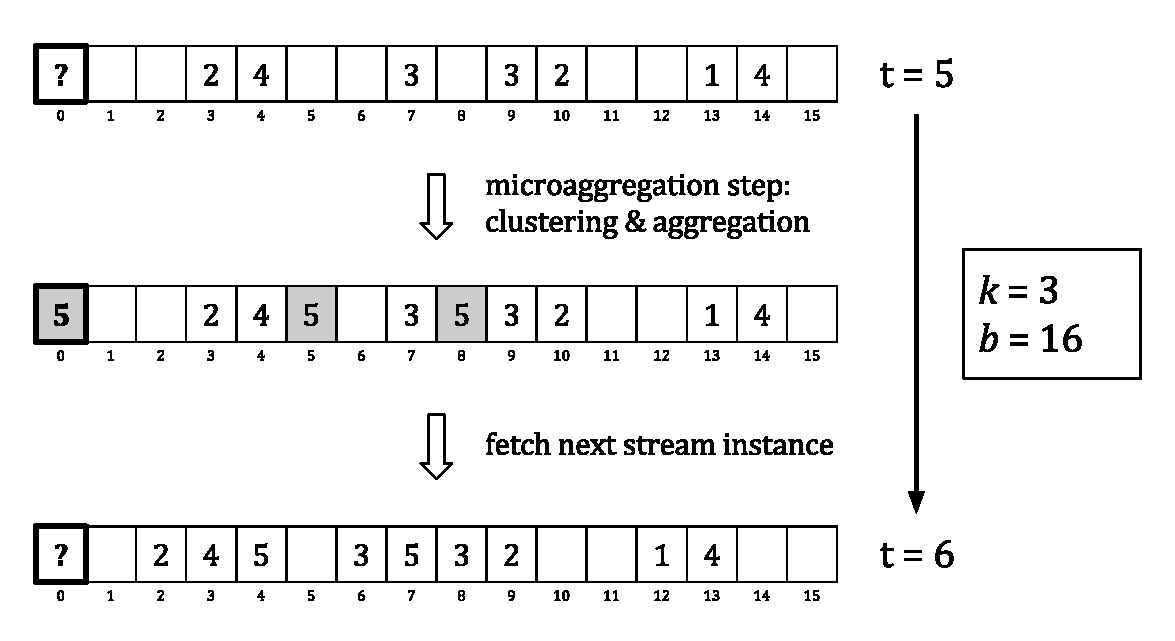
\includegraphics[width=0.9\textwidth]{figures/microaggregation-schematic-1.pdf}
	\caption[Streaming KNN-based microaggregation.]{$k$-Nearest Neighbours based microaggregation schematic of a whole processing step (from time $t=5$ to $t=6$). The \textit{target} instance at the top of the buffer (position 0) is anonymized by aggregating the values of its attributes with the other instances of the cluster, highlighted with a gray background. Afterwards, it is flushed out of the buffer and a new instance is received.}
	\label{fig:microaggregation-schematic-1}
\end{figure}

Our proposal is to use a $k$-Nearest Neighbours (KNN) algorithm to \textit{continuously} partition the sliding window and be able to provide anonymized instances much faster, by building just \textit{one} cluster each time a new instance is requested to the filter. The records in this single cluster are then aggregated and the target instance is returned. The computational cost of this approach is quite lower than that of the MDAV and $\mu$-Approx heuristics, as long as the sliding window size remains relatively small.

The idea of this partition procedure, formally explained in~\alref{al:KNN-partition}, is to calculate, for all instances not yet anonymized, the distance to the target ($\tau$), keeping track of the $k-1$ nearest ones. If an instance is closer than the current furthest, the latter is removed from the cluster and the former is added. At the end of the buffer traversal, together with $\tau$, the instances that have been kept will form the next cluster of the stream partition. The distance metric used is the same than that used by the default disclosure risk estimator (see~\sref{Implementation:Estimators:RecordLinker} and~\procref{al:distance}).

The KNN algorithm uses a \textit{priority queue}\footnote{A \textit{max-heap} is used to keep the greatest element on top of the queue.} to hold the $k-1$ nearest neighbours to the target, $\tau$. The queue works over \textit{distance-index} pairs $\langle d, i\rangle$, but is actually indexed by $d$, holding the greatest value on the top of the queue. This way, it is very cheap (constant time) to know whether a given instance $x$ is closer than the current furthest instance from $\tau$. Insertions are also cheap, with an upper bound cost of $O(\mathrm{log}(k))$.

The overall cost of the procedure, when implemented with a priority queue, depends on the amount of instances $n$ being processed, the size $b$ of the sliding window and the size $k$ of the clusters and its upper bound is $O(n \cdot b \cdot \mathrm{log}(k))$.

\begin{algorithm}
\KwData{$W', A$}
\KwResult{a \textit{cluster} $\mathcal{C}$ of $k$ instance indexes such that $\mathrm{index}(\tau) \in \mathcal{C}$}
\Begin{
	$\tau \leftarrow w_0'$\;
	$\mathcal{C} \leftarrow \emptyset \cup \tau$\;
	$Q \leftarrow$ PriorityQueue$\langle$DistanceIndexPair$\rangle$()\;
	\For{$ x \in W', x \notin A $}{
		$d \leftarrow \mathrm{dist}(x,\tau)$\;
		$p \leftarrow$ DistanceIndexPair($d$, index($x$))\;
		\eIf{$\vert Q \vert < k$}{
			$Q \leftarrow Q \cup p$\;
		}{
			\If{$d < Q$.peek()}{
				$Q.poll()$\;
				$Q \leftarrow Q \cup p$\;
			}
		}
	}
	\For{$p \in Q$}{
		$\mathcal{C} \leftarrow \mathcal{C} \cup p.index()$\;
	}
	\KwRet $\mathcal{C}$\;
}
\caption{KNNPartition\label{al:KNN-partition}}
\end{algorithm}

\subsubsection{Aggregation}

After a cluster has been obtained from the previous partition step, the instances of the cluster are aggregated, this is, the values of their attributes are imputed with the values of the \textit{centroid} of the cluster. For each attribute, the arithmetic mean (in the case that the attribute is numeric) or the mode (if the attribute is nominal) are calculated over the instances of the cluster. We do not provide any figure or algorithm concerning this step, due its simplicity.

The computational cost of the aggregation step is directly related to the size $k$ of the clusters and can be approximated to $\Theta(n \cdot 2 \cdot m \cdot k)$, where $n$ is the number of instances processed and $m$ is the number of attributes. This is: for each of the $m$ attributes, a first traversal over the $k$ instances in the cluster is done to compute the averages and a second one to impute the values of the centroid found. If we add together both steps, we found the total cost of the algorithm: $O(n \cdot (b \cdot \mathrm{log}(k) + 2 \cdot m \cdot k))$. However, given that $m \ll n$ and $k \ll b, n$, the overall cost of this microaggregation implementation is actually dominated by the cost of the clustering step: $O(n \cdot b \cdot \mathrm{log}(k))$.

\subsection{Summary}
\label{Implementation:Microaggregation:Summary}

The \texttt{MicroAggregationFilter} implements a microaggregation algorithm based on a KNN clustering for the partition step and a basic centroid aggregation scheme. \fref{fig:microaggregation-schematic-2} shows a complete execution for a given target instance and~\tref{table:microaggregation-summary} summarizes the main properties of this SDC method.

\begin{figure}[h]
	\centering
	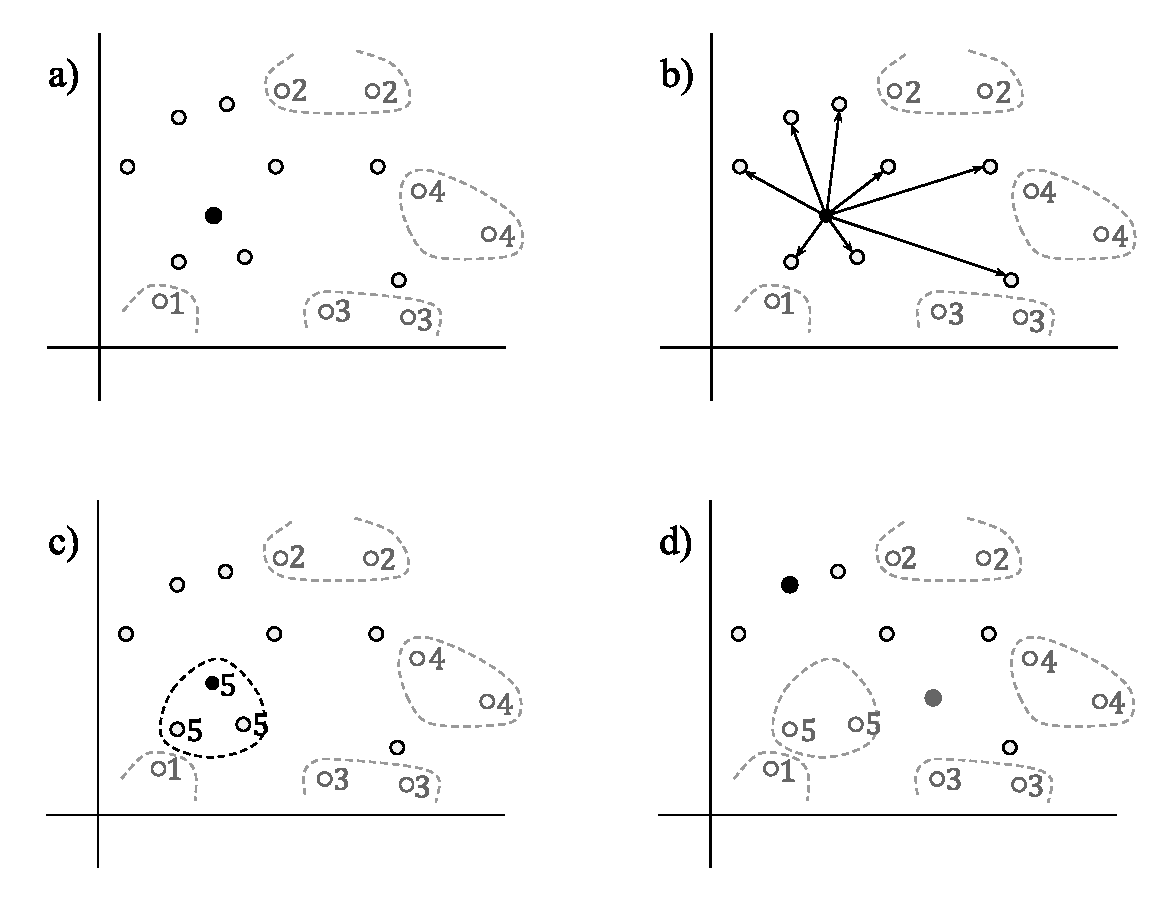
\includegraphics[width=.9\textwidth]{figures/microaggregation-schematic-2.pdf}
	\caption[KNN microaggregation, step by step.]{KNN-based microaggregation ($k = 3$, $b = 16$). Firstly, the target instance (black) is not anonymized (a). Distances to the remaining non-anonymized instances are calculated (b) and a cluster is formed with the $k-1$ nearest ones (c). After aggregating the records in the cluster, the target instance is streamed out, a new instance (grey) is received and a new target is selected (d).}
	\label{fig:microaggregation-schematic-2}
\end{figure}

\begin{table}[h]
	\centering
	\begin{tabular}{@{}ll@{}}
	\toprule
	\multicolumn{2}{l}{\textbf{MicroAggregationFilter}}                             \\ \midrule
	\textbf{Parameters}   & $k$ (cluster size), $b$ (buffer size)                   \\
	\textbf{Type of data} & Heterogeneous (both numeric and categorical attributes) \\
	\textbf{Cost}         & $O(n \cdot b \cdot \mathrm{log}(k))$                    \\ \bottomrule
	\end{tabular}
	\caption{\texttt{MicroAggregationFilter} summary.}
	\label{table:microaggregation-summary}
\end{table}